%%%%%%%%%%%%%%%%%%%%%%%%%%%%%%%%%%%%%%%%%%%%%%%%%%%%%%%%%%%%%%%%%%%%%%%%%%%%%%%%
% TUM-Vorlage: Präsentation
%%%%%%%%%%%%%%%%%%%%%%%%%%%%%%%%%%%%%%%%%%%%%%%%%%%%%%%%%%%%%%%%%%%%%%%%%%%%%%%%
%
% Rechteinhaber:
%     Technische Universität München
%     https://www.tum.de
% 
% Gestaltung:
%     ediundsepp Gestaltungsgesellschaft, München
%     http://www.ediundsepp.de
% 
% Technische Umsetzung:
%     eWorks GmbH, Frankfurt am Main
%     http://www.eworks.de
%
%%%%%%%%%%%%%%%%%%%%%%%%%%%%%%%%%%%%%%%%%%%%%%%%%%%%%%%%%%%%%%%%%%%%%%%%%%%%%%%%


%%%%%%%%%%%%%%%%%%%%%%%%%%%%%%%%%%%%%%%%%%%%%%%%%%%%%%%%%%%%%%%%%%%%%%%%%%%%%%%%
% Zur Wahl des Seitenverhältnisses bitte einen der beiden folgenden Befehle
% auskommentieren und den ausführen lassen:
\documentclass[t]{beamer}
\usepackage[
    orientation=landscape,
    size=custom,
    width=25.4,
    height=19.05,
    scale=0.63 % erzeugt 16pt Schriftgröße
]{beamerposter}

\newcommand{\PraesentationSchriftgroesseSehrGross}{\fontsize{30}{45}}
\newcommand{\PraesentationSchriftgroesseGross}{\fontsize{22}{33}}
\newcommand{\PraesentationSchriftgroesseNormal}{\fontsize{16}{29}}
\newcommand{\PraesentationSchriftgroesseKlein}{\fontsize{12}{18}}
\newcommand{\PraesentationSchriftgroesseDreizeiler}{\fontsize{7}{10}}
\newcommand{\PraesentationSchriftgroesseAufzaehlungszeichen}{\fontsize{10}{8}}

\newcommand{\PraesentationAbstandAbsatz}{22.1pt}
\newcommand{\PraesentationPositionKorrekturOben}{0cm}
\newcommand{\PraesentationBeispieleSchriftgroessen}{30 | 22 | 16 | 12}
\usepackage[utf8]{inputenc}
\usepackage[T1]{fontenc} % Zeichensatzkodierung

\usepackage{calc} % Berechnungen

\usepackage[ngerman]{babel} % Deutsche Lokalisierung
\usepackage{graphicx} % Grafiken
\usepackage[absolute, overlay]{textpos} % Positionierung

% Silbentrennung:
\usepackage{hyphenat}
%\tolerance 2414
%\hbadness 2414
%\emergencystretch 1.5em
%\hfuzz 0.3pt
%\widowpenalty=10000     % Hurenkinder
%\clubpenalty=10000      % Schusterjungen
%\vfuzz \hfuzz

% Euro-Symbol:
\usepackage[gen]{eurosym}
\DeclareUnicodeCharacter{20AC}{\euro{}}

% Schriftart Helvetica:
\usepackage[scaled]{helvet}
\renewcommand{\familydefault}{\sfdefault}

\usepackage{mathptmx} % skalierbare Formelschriften

\usepackage{tabularx}

\usepackage{multicol} % mehrspaltiger Text

\usepackage{tikz}
\usetikzlibrary{arrows, shapes, shapes.multipart, trees, positioning,
    backgrounds, fit, matrix, external}

% Diagramme:
\usepackage{pgfplots}
\pgfplotsset{compat=default}

% Erweiterbare Fusszeile:
\newcommand{\PraesentationFusszeileZusatz}{}

\usepackage{bookmark} % Lesezeichen

% Unterdrückung layoutbedingter Warnungen
\usepackage[immediate]{silence}
\WarningFilter[layout]{lastpage}{Rerun to get the references right} % Gesamtseitenzahl
\WarningFilter[layout]{latex}{Label(s) may have changed.} % Referenz auf letzte Seite
\WarningFilter[layout]{pgfplots}{running in backwards compatibility mode (unsuitable tick labels; missing features).} % Labelerstellung ab Version 1.17 nicht abwärtskompatibel
\WarningFilter[layout]{latex}{There were undefined references}
\WarningFilter[layout]{latex}{Reference `PraesentationDiagramm} % Erstellung einer Legende außerhalb des Diagrammbereichs

% Debugging:
%\DeactivateWarningFilters[layout] % Unterdrückte Warnungen einschalten % Seitenverhältnis 4:3
% %\documentclass[aspectratio=169]{beamer}
\documentclass[t,aspectratio=169]{beamer}
\usepackage[
    orientation=landscape,
    size=custom,
    width=25.4,
    height=14.2875,
    scale=0.5
]{beamerposter}

\newcommand{\PraesentationSchriftgroesseSehrGross}{\fontsize{25}{38}}
\newcommand{\PraesentationSchriftgroesseGross}{\fontsize{18}{27}}
\newcommand{\PraesentationSchriftgroesseNormal}{\fontsize{14}{21}}
\newcommand{\PraesentationSchriftgroesseKlein}{\fontsize{11}{17}}
\newcommand{\PraesentationSchriftgroesseDreizeiler}{\fontsize{7}{10}}
\newcommand{\PraesentationSchriftgroesseAufzaehlungszeichen}{\fontsize{10}{8}}

\newcommand{\PraesentationAbstandAbsatz}{18pt}
\newcommand{\PraesentationPositionKorrekturOben}{-1cm}
\newcommand{\PraesentationBeispieleSchriftgroessen}{25 | 18 | 14 | 11}
\usepackage[utf8]{inputenc}
\usepackage[T1]{fontenc} % Zeichensatzkodierung

\usepackage{calc} % Berechnungen

\usepackage[ngerman]{babel} % Deutsche Lokalisierung
\usepackage{graphicx} % Grafiken
\usepackage[absolute, overlay]{textpos} % Positionierung

% Silbentrennung:
\usepackage{hyphenat}
%\tolerance 2414
%\hbadness 2414
%\emergencystretch 1.5em
%\hfuzz 0.3pt
%\widowpenalty=10000     % Hurenkinder
%\clubpenalty=10000      % Schusterjungen
%\vfuzz \hfuzz

% Euro-Symbol:
\usepackage[gen]{eurosym}
\DeclareUnicodeCharacter{20AC}{\euro{}}

% Schriftart Helvetica:
\usepackage[scaled]{helvet}
\renewcommand{\familydefault}{\sfdefault}

\usepackage{mathptmx} % skalierbare Formelschriften

\usepackage{tabularx}

\usepackage{multicol} % mehrspaltiger Text

\usepackage{tikz}
\usetikzlibrary{arrows, shapes, shapes.multipart, trees, positioning,
    backgrounds, fit, matrix, external}

% Diagramme:
\usepackage{pgfplots}
\pgfplotsset{compat=default}

% Erweiterbare Fusszeile:
\newcommand{\PraesentationFusszeileZusatz}{}

\usepackage{bookmark} % Lesezeichen

% Unterdrückung layoutbedingter Warnungen
\usepackage[immediate]{silence}
\WarningFilter[layout]{lastpage}{Rerun to get the references right} % Gesamtseitenzahl
\WarningFilter[layout]{latex}{Label(s) may have changed.} % Referenz auf letzte Seite
\WarningFilter[layout]{pgfplots}{running in backwards compatibility mode (unsuitable tick labels; missing features).} % Labelerstellung ab Version 1.17 nicht abwärtskompatibel
\WarningFilter[layout]{latex}{There were undefined references}
\WarningFilter[layout]{latex}{Reference `PraesentationDiagramm} % Erstellung einer Legende außerhalb des Diagrammbereichs

% Debugging:
%\DeactivateWarningFilters[layout] % Unterdrückte Warnungen einschalten % Seitenverhältnis 16:9
%%%%%%%%%%%%%%%%%%%%%%%%%%%%%%%%%%%%%%%%%%%%%%%%%%%%%%%%%%%%%%%%%%%%%%%%%%%%%%%%


%%%%%%%%%%%%%%%%%%%%%%%%%%%%%%%%%%%%%%%%%%%%%%%%%%%%%%%%%%%%%%%%%%%%%%%%%%%%%%%%
%%%%%%%%%%%%%%%%%%%%%%%%%%%%%%%%%%%%%%%%%%%%%%%%%%%%%%%%%%%%%%%%%%%%%%%%%%%%%%%%
% TUM-Vorlage: Personenspezifische Informationen
%%%%%%%%%%%%%%%%%%%%%%%%%%%%%%%%%%%%%%%%%%%%%%%%%%%%%%%%%%%%%%%%%%%%%%%%%%%%%%%%
%
% Rechteinhaber:
%     Technische Universität München
%     https://www.tum.de
% 
% Gestaltung:
%     ediundsepp Gestaltungsgesellschaft, München
%     http://www.ediundsepp.de
% 
% Technische Umsetzung:
%     eWorks GmbH, Frankfurt am Main
%     http://www.eworks.de
%
%%%%%%%%%%%%%%%%%%%%%%%%%%%%%%%%%%%%%%%%%%%%%%%%%%%%%%%%%%%%%%%%%%%%%%%%%%%%%%%%

% Für die Person anpassen:

\newcommand{\PersonTitel}{}
\newcommand{\PersonVornameAl}{Alex}
\newcommand{\PersonNachnameHo}{Hocks}
\newcommand{\PersonVornameJa}{Jan}
\newcommand{\PersonNachnameHa}{Hampe}
\newcommand{\PersonVornameJo}{Johannes}
\newcommand{\PersonNachnameRi}{Riemenschneider}
\newcommand{\PersonStadt}{Garching}
\newcommand{\PersonAdresse}{%
    %@Adresse@\\%
    @85748@~\PersonStadt%
}
\newcommand{\PersonTelefon}{@Telefon@}
\newcommand{\PersonFax}{@Fax@}
\newcommand{\PersonEmail}{@E-Mail@}
\newcommand{\PersonWebseite}{@Web@}

\newcommand{\FakultaetAnsprechpartner}{@Ansprechpartner@}
\newcommand{\LehrstuhlName}{@Lehrstuhlname@}

\newcommand{\EinstellungBankName}{Bayerische Landesbank}
\newcommand{\EinstellungBankIBAN}{DE10700500000000024866}
\newcommand{\EinstellungBankBIC}{BYLADEMM}
\newcommand{\EinstellungSteuernummer}{143/241/80037}
\newcommand{\EinstellungUmsatzsteuerIdentifikationsnummer}{DE811193231}

\hyphenation{} % eigene Silbentrennung                    % !!! DATEI ANPASSEN !!!
%%%%%%%%%%%%%%%%%%%%%%%%%%%%%%%%%%%%%%%%%%%%%%%%%%%%%%%%%%%%%%%%%%%%%%%%%%%%%%%%


\renewcommand{\PersonTitel}{Dr. rer. nat.}
\newcommand{\Datum}{\today}

\renewcommand{\PraesentationFusszeileZusatz}{| kann beliebig erweitert werden | Infos mit Strich trennen}

\title{Titel der Präsentation bearbeiten}
\author{\PersonTitel{} \PersonVorname{} \PersonNachname}
\institute[]{\UniversitaetName \\ \FakultaetName \\ \LehrstuhlName}
\date[\Datum]{München, 27. März 2015}
\subject{Thema der Präsentation}


%%%%%%%%%%%%%%%%%%%%%%%%%%%%%%%%%%%%%%%%%%%%%%%%%%%%%%%%%%%%%%%%%%%%%%%%%%%%%%%%
%%%%%%%%%%%%%%%%%%%%%%%%%%%%%%%%%%%%%%%%%%%%%%%%%%%%%%%%%%%%%%%%%%%%%%%%%%%%%%%%
% EINSTELLUNGEN
%%%%%%%%%%%%%%%%%%%%%%%%%%%%%%%%%%%%%%%%%%%%%%%%%%%%%%%%%%%%%%%%%%%%%%%%%%%%%%%%

% Allgemein:
\newcommand{\AllgemeinGestalter}{ediundsepp Gestaltungsgesellschaft}
\newcommand{\AllgemeinErsteller}{eWorks GmbH}

% Universität:
\newcommand{\UniversitaetName}{Technische Universität München}
\newcommand{\UniversitaetAbkuerzung}{TUM}
\newcommand{\UniversitaetWebseite}{www.tum.de}
\newcommand{\UniversitaetLogoBreite}{19mm}
\newcommand{\UniversitaetLogoHoehe}{1cm}

\newcommand{\UniversitaetAdresse}{%
    Arcisstraße~21\\%
    80333~München%
}

% Fakultät:
\newcommand{\FakultaetName}{@Fakultät@}




% Seitenränder:
\newcommand{\SeitenrandOben}{20mm}
\newcommand{\SeitenrandRechts}{20mm}
\newcommand{\SeitenrandLinks}{25mm}
\newcommand{\SeitenrandUnten}{10mm}

% Falzmarken:
\newcommand{\FalzmarkeOben}{87mm}
\newcommand{\FalzmarkeMitte}{148.5mm}
\newcommand{\FalzmarkeUnten}{192mm}
\newcommand{\FalzmarkeBreite}{2mm}
\newcommand{\FalzmarkeDicke}{0.3pt}
\newcommand{\FalzmarkePositionLinks}{7mm}


% Adressfeld:
\newcommand{\AdressfeldHoehe}{45mm}
\newcommand{\AdressfeldBreite}{85mm}
\newcommand{\AdressfeldAbsenderSchriftgroesse}{7.5pt}
\newcommand{\AdressfeldEmpfaengerSchriftgroesse}{11pt}
\newcommand{\AdressfeldEmpfaengerZeilenabstand}{15pt}

% Text:
\newcommand{\TextOben}{77.5mm}
\newcommand{\TextSchriftgroesse}{11pt}
\newcommand{\TextZeilenabstand}{15pt}

% Fusszeile:
\newcommand{\FusszeilePositionOben}{271mm}
\newcommand{\FusszeileBreite}{165mm}
\newcommand{\FusszeileHoehe}{16.5mm}
\newcommand{\FusszeileZwischenabstand}{2mm}
\newcommand{\FusszeileBreiteGross}{44mm}
\newcommand{\FusszeileBreiteKlein}{35.0mm}
\newcommand{\FusszeileSeitennummerAbstand}{7.7mm}
\newcommand{\FusszeileSchriftgroesse}{7.5pt}
\newcommand{\FusszeileZeilenabstand}{8pt}


%%%%%%%%%%%%%%%%%%%%%%%%%%%%%%%%%%%%%%%%%%%%%%%%%%%%%%%%%%%%%%%%%%%%%%%%%%%%%%%%
% DOKUMENT
%%%%%%%%%%%%%%%%%%%%%%%%%%%%%%%%%%%%%%%%%%%%%%%%%%%%%%%%%%%%%%%%%%%%%%%%%%%%%%%%

\usepackage[a4paper,
    top=\SeitenrandOben - 7mm,
    bottom=\SeitenrandUnten,
    inner=\SeitenrandLinks,
    outer=\SeitenrandRechts,
    foot=\FusszeileHoehe - 1mm,
    head=35mm,
    includefoot
]{geometry}

\textblockorigin{\SeitenrandLinks}{\SeitenrandOben} % Ursprung für Positionierung

\newcommand{\RechnungTitel}{Rechnung Nr. \RechnungNummer}

% PDF-Einstellungen:
\usepackage{hyperref}
\hypersetup{
    hidelinks,
    pdfauthor={\PersonVorname{} \PersonNachname},
    pdftitle={\RechnungTitel},
    pdfproducer={\AllgemeinErsteller},
    pdfcreator={\AllgemeinGestalter}
}

\renewcommand*{\raggedsignature}{\raggedright}

\makeatletter
    \@setplength{bfoldmarklength}{\FalzmarkeBreite}
    \@setplength{bfoldmarkvpos}{\FalzmarkeUnten}
    \@setplength{firstfoothpos}{\SeitenrandLinks - 2pt}
    \@setplength{firstfootvpos}{\FusszeilePositionOben}
    \@setplength{firstfootwidth}{\FusszeileBreite}
    \@setplength{foldmarkhpos}{\FalzmarkePositionLinks}
    \@setplength{foldmarkthickness}{\FalzmarkeDicke}
    \@setplength{mfoldmarklength}{\FalzmarkeBreite}
    \@setplength{mfoldmarkvpos}{\FalzmarkeMitte}

    \@setplength{refaftervskip}{\TextZeilenabstand}
    \@setplength{refvpos}{\TextOben}
    \@setplength{sigbeforevskip}{\baselineskip}
    \@setplength{sigindent}{0mm}
    \@setplength{subjectaftervskip}{\baselineskip + 1pt}

    \@setplength{tfoldmarklength}{\FalzmarkeBreite}
    \@setplength{tfoldmarkvpos}{\FalzmarkeOben}
\makeatother

\KOMAoptions{
    fontsize=\TextSchriftgroesse,
    foldmarks=BMpTv,
    firsthead=false,
    backaddress=no,
    addrfield=no,
    fromalign=false
}

\setkomavar{fromname}{\UniversitaetName}
\setkomavar{fromaddress}{\PersonAdresse}
\addtokomafont{backaddress}{\fontsize{\AdressfeldAbsenderSchriftgroesse}{\AdressfeldAbsenderSchriftgroesse}\selectfont}
\addtokomafont{toaddress}{\fontsize{\AdressfeldEmpfaengerSchriftgroesse}{\AdressfeldEmpfaengerZeilenabstand}\selectfont}

\newcommand{\RuecksendeadresseTrenner}{~| \ignorespaces}

\AtBeginLetter{%
    % Logo:
    \begin{textblock*}{\UniversitaetLogoBreite}[1,0](\textwidth, 0cm)%
        \raggedleft%
        
\includegraphics{./Ressourcen/_Bilder/Universitaet_Logo_RGB.pdf}%
    \end{textblock*}%
    \setlength{\baselineskip}{\TextZeilenabstand}%
    \setlength{\parindent}{0mm} % keine Einrückung am Absatzanfang
    \setlength{\parskip}{\baselineskip} % einzeiliger Abstand nach Absätzen
    \setlength{\tabcolsep}{1mm} % Spaltenabstand in Tabellen
    % Empfängerfenster:
    \begin{textblock*}{\AdressfeldBreite}[0,0](0cm, 15mm)%
        \raggedbottom\raggedright
        \begin{spacing}{.85}%
        {
            \usekomafont{backaddress}%
            \let\\\RuecksendeadresseTrenner% Umdefinieren von "\\" zu "~| "
            \Absender%
        } \\
        \end{spacing}
        \vspace*{5.5pt}
        \usekomafont{toaddress}%
        \EmpfaengerAdresse
    \end{textblock*}
}

\KOMAoptions{refline=dateleft}
\setkomavar{date}{\Datum}
\setkomavar{place}{\PersonStadt}
\setkomafont{subject}{\bfseries}
\setkomavar{subject}{%
    \RechnungTitel\newline%
    BKZ-Nr. \RechnungBearbeitungskennzeichen~--~geben Sie immer diese Nummer mit an!%
}
\setkomavar{signature}{\PersonVorname~\PersonNachname}

%\setkomavar*{enclseparator}{Anlage\vspace{-3em}}

\renewcommand*{\closing}[1]{#1\newline\newline\usekomavar{signature}\newline}
\setkomavar{enclseparator}[Anlage]{~}
\renewcommand{\encl}[1]{\newline{}Anlage~#1}

\KOMAoptions{firstfoot=true}
\setkomafont{pagefoot}{\sffamily\fontsize{7.5pt}{8pt}\selectfont}
\renewcommand{\pagemark}{%
\begin{textblock*}{3em}[1,1](\paperwidth - \SeitenrandLinks - \SeitenrandRechts + \FusszeileSeitennummerAbstand + 3mm, \paperheight - \SeitenrandOben - \SeitenrandUnten)%
    \raggedleft\normalfont\hfill\usekomafont{pagefoot}\thepage\,/\,\pageref*{LastPage}%
\end{textblock*}%
}

\setkomavar{firstfoot}{
    \TabPositions{2em}%
    \begin{minipage}[t][\FusszeileHoehe][t]{\FusszeileBreiteGross}%
        \usekomafont{pagefoot}%
        \textbf{\UniversitaetName}%
        \newline%
        \FakultaetName%
        \newline%
        \LehrstuhlName%
    \end{minipage}%
    \hspace*{\FusszeileZwischenabstand}%
    \begin{minipage}[t][\FusszeileHoehe][t]{\FusszeileBreiteGross}%
        \raggedright\usekomafont{pagefoot}%
        \textbf{\FakultaetAnsprechpartner}\newline%
        \PersonAdresse%
    \end{minipage}%
    \hspace*{\FusszeileZwischenabstand}%
    \begin{minipage}[t][\FusszeileHoehe][t]{\FusszeileBreiteKlein}%
        \raggedright\usekomafont{pagefoot}%
        Tel.\tab{\PersonTelefon}%
        \def\temp{\PersonFax}\ifx\temp\empty%
        \else%
          \newline Fax\tab{\PersonFax}%
        \fi%
        \newline\newline%
        \PersonEmail\newline%
        \href{http://\PersonWebseite}{\PersonWebseite}\newline%
        \href{http://\UniversitaetWebseite}{\UniversitaetWebseite}%
    \end{minipage}%
    \hspace*{\FusszeileZwischenabstand}%
    \begin{minipage}[t][\FusszeileHoehe][t]{\FusszeileBreiteKlein}%
        \raggedright\usekomafont{pagefoot}%
        \EinstellungBankName\newline%
        IBAN-Nr.: \EinstellungBankIBAN\newline%
        BIC: \EinstellungBankBIC\newline%
        Steuer-Nr.: \EinstellungSteuernummer\newline%
        USt-IdNr.: \EinstellungUmsatzsteuerIdentifikationsnummer\newline%
    \end{minipage}%
    \pagemark%
}

\pagestyle{plain.scrheadings}
\setlength{\headsep}{35mm}
\ohead*{
    \begin{textblock*}{\UniversitaetLogoBreite}[1,0](\textwidth, 0cm)%
        \raggedleft%
        
\includegraphics{./Ressourcen/_Bilder/Universitaet_Logo_RGB.pdf}%
    \end{textblock*}%
}

% Tabellen
\usepackage{array}
\newcolumntype{L}[1]{>{\raggedright\let\newline\\\arraybackslash\hspace{0pt}}p{#1}}
\newcolumntype{R}[1]{>{\raggedleft\let\newline\\\arraybackslash\hspace{0pt}}p{#1}}

\newcommand{\RechnungTabelleLinie}{\specialrule{0.3pt}{1mm}{1mm}}
\newcommand{\RechnungTabelleZeile}[6]{%
    \hspace{1mm}#1 & #2 & #3 & #4 & #5 & #6 \\
}
\NewEnviron{RechnungTabelle}[3]{
    \begin{tabularx}{\textwidth}{
        @{\extracolsep{\fill}}
        L{12mm - \tabcolsep}
        L{35mm - \tabcolsep - \tabcolsep}
        L{46mm - \tabcolsep - \tabcolsep}
        l
        R{27mm - \tabcolsep - \tabcolsep}
        R{27mm - \tabcolsep}
    }
    \specialrule{0.3pt}{0mm}{1mm}
    \hspace{1mm}{\bfseries Pos.} & {\bfseries Art.-Nr. (o.ä.)} & {\bfseries Bezeichnung} & {\bfseries Menge} & {\bfseries Einzelpreis} & {\bfseries Summe} \\
    \specialrule{0.6pt}{2mm}{1mm}
    \noindent
\BODY
    \specialrule{0.6pt}{1mm}{1mm}
    \multicolumn{5}{l}{\noindent Gesamt Netto} & #1 \\
    \specialrule{0.3pt}{2mm}{1mm}
    \multicolumn{5}{l}{\noindent zzgl. 19\% USt.} & #2 \\
    \specialrule{0.3pt}{2mm}{1mm}
    \multicolumn{5}{l}{\bfseries\noindent Gesamtbetrag} & {\bfseries #3} \\
    \specialrule{0.6pt}{2mm}{0mm}
    \end{tabularx}
    \vspace*{3pt}
}

\begin{document}
\raggedright
\begin{letter}{}
\opening{}
 % !!! NICHT ENTFERNEN !!!
%%%%%%%%%%%%%%%%%%%%%%%%%%%%%%%%%%%%%%%%%%%%%%%%%%%%%%%%%%%%%%%%%%%%%%%%%%%%%%%%


%%%%%%%%%%%%%%%%%%%%%%%%%%%%%%%%%%%%%%%%%%%%%%%%%%%%%%%%%%%%%%%%%%%%%%%%%%%%%%%%
% FOLIENSTIL: Standard
\PraesentationMasterStandard

\PraesentationTitelseite % Fügt die Startseite ein


%%%%%%%%%%%%%%%%%%%%%%%%%%%%%%%%%%%%%%%%%%%%%%%%%%%%%
%% Beispielfolien                                  %%
\usepackage{tikz}
\usepackage{graphicx}
\usepackage{listings}
\usepackage{media9}

\addmediapath{./videos/}
%%%%%%%%%%%%%%%%%%%%%%%%%%%%%%%%%%%%%%%%%%%%%%%%%%%%%%%%%%%%%%%%%%%%%%%%%%%%%%%%
% TUM-Vorlage: Präsentation - Beispiele
%%%%%%%%%%%%%%%%%%%%%%%%%%%%%%%%%%%%%%%%%%%%%%%%%%%%%%%%%%%%%%%%%%%%%%%%%%%%%%%%


\begin{frame}
\frametitle{2 Dimensional Force Calculation}
	\begin{textblock}{0}(0,3.5)
	\begin{tikzpicture}[ultra thick]
	
	\foreach \Point in {(0.05,-0.05), (7.95,3.95)}{
		\node at \Point {\textbullet};
	}
	
	\draw[thick]	(0,0) -- (8,4);
	\draw[thick]    (0,0) -- (8,0);
	
	\draw (1.5,0) arc (0:atan(4/8)):1.5)
	node[pos = 0.5, right = 2pt]{\large $\theta$};
	
	\draw [decorate, decoration = {brace, raise = 9pt, amplitude = 9pt}] 	(8,0) --  (0,0)
	node [pos = 0.5, below = 18 pt]{\large $\Delta x$};
	\draw [decorate, decoration = {brace, raise = 9pt, amplitude = 9pt}] (8,4) --  (8, 0)
	node [pos = 0.5, right = 18 pt]{\large $\Delta y$};
	\end{tikzpicture}
	\end{textblock}
	
	\begin{textblock}{7}(6,4)
		\large
		\begin{equation}
			\Delta x = x_2 - x_1
		\end{equation}
		\begin{equation}
			\Delta y = y_2 - y_1
		\end{equation}
		\begin{equation}
			|F| = \frac{m_1 m_2}{\Delta x^2 + \Delta y^2}
		\end{equation}
		
	\end{textblock}´

	\begin{textblock}{10}(2, 10)
		\large
		\begin{equation}
			F_x = \cos(\theta) \cdot |F| = \Delta x \cdot \frac{m_1 m_2}{\left( \Delta x^2 + \Delta y^2 \right)^{3/2}}
		\end{equation}
		\begin{equation}
			F_y = \sin(\theta) \cdot |F| = \Delta y \cdot \frac{m_1 m_2}{\left( \Delta x^2 + \Delta y^2 \right)^{3/2}}
		\end{equation}
		
		
	\end{textblock}
	
\end{frame}

\begin{frame}[fragile]
	\frametitle{Utilizing $F_{ij} = -F_{ji}$}
	\large 
	The naive approach ($n\cdot (n-1)$ Force calculations):\\
	%\vspace{-0.1cm}
	\begin{Verbatim}
for all Particles p:
	for all Particles p'!=p:
		computeF(p,p')
	\end{Verbatim}
	\centering
	\begin{tikzpicture}[ultra thick]
		\foreach \Point in {(0,0), (1, 4), (5,3), (8,1)}{
			\node at \Point {\textbullet};
		}
		\visible<1>{
			\draw[->, gray]{(0,0) -- (0.24, 0.97)};
			\draw[->, gray]{(0,0) -- (0.86, 0.51)};
			\draw[->, gray]{(0,0) -- (0.99, 0.124)};
			%\draw[->, gray, scale=0.24]{(0,0) -- (1,4)};
			%\draw[->, gray, scale=0.17]{(0,0) -- (5,3)};
			%\draw[->, gray, scale=0.125]{(0,0) -- (8,1)};
		}
		
		\visible<2>{
			\draw[->, gray]{(1,4) -- (0.76, 3.03)};
			\draw[->, gray]{(1,4) -- (1.97, 3.76)};
			\draw[->, gray]{(1,4) -- (1.92, 3.61)};
		}
		\visible<3>{
			\draw[->, gray]{(5,3) -- (4.14, 2.49)};	
			\draw[->, gray]{(5,3) -- (4.03, 3.24)};	
			\draw[->, gray]{(5,3) -- (5.83, 2.45)};	
		}
	
		\visible<4>{
			\draw[->, gray]{(8,1) -- (7.01, 0.88)};	
			\draw[->, gray]{(8,1) -- (7.08, 1.39)};	
			\draw[->, gray]{(8,1) -- (7.17, 1.55)};	
		}
	%\begin{textblock}{7}(5,7)
	%	\large
	%	\visible<5>{$n\cdot(n-1) \text{computations of F necessary}$} hässlich aber sonst nimmt er es nicht
	%\end{textblock}
		
	\end{tikzpicture}
	\end{frame}
	
	\begin{frame}[fragile]
		\frametitle{Utilizing $F_{ij} = -F_{ji}$}
		\large 
		A better approach ($\frac{1}{2} n\cdot (n-1)$ Force calculations):\\
		\begin{Verbatim}
for all ParticlePairs (p,p'):
	computeF(p,p')
		\end{Verbatim}
	\centering
\begin{tikzpicture}[ultra thick]
\foreach \Point in {(0,0), (1, 4), (5,3), (8,1)}{
	\node at \Point {\textbullet};
}
\visible<1>{\draw[gray] (0,0) -- (1,4);}
\visible<2>{\draw[gray] (1,4) -- (5,3);}
\visible<3>{\draw[gray] (5,3) -- (8,1);}
\visible<4>{\draw[gray] (0,0) -- (5,3);}
\visible<5>{\draw[gray] (0,0) -- (8,1);}
\end{tikzpicture}
	
\end{frame}

%%%%%%%%%%%%%%%%%%%%%%%%%%%%%%%%%%%%%%%%%%%%%%%%%%%%%
%% Folie: Gültigkeit der Masterfolien              %%
%%%%%%%%%%%%%%%%%%%%%%%%%%%%%%%%%%%%%%%%%%%%%%%%%%%%%

\begin{frame}
\frametitle{Refactoring}
\vspace{-0.5cm}
´\begin{figure}
	\centering
	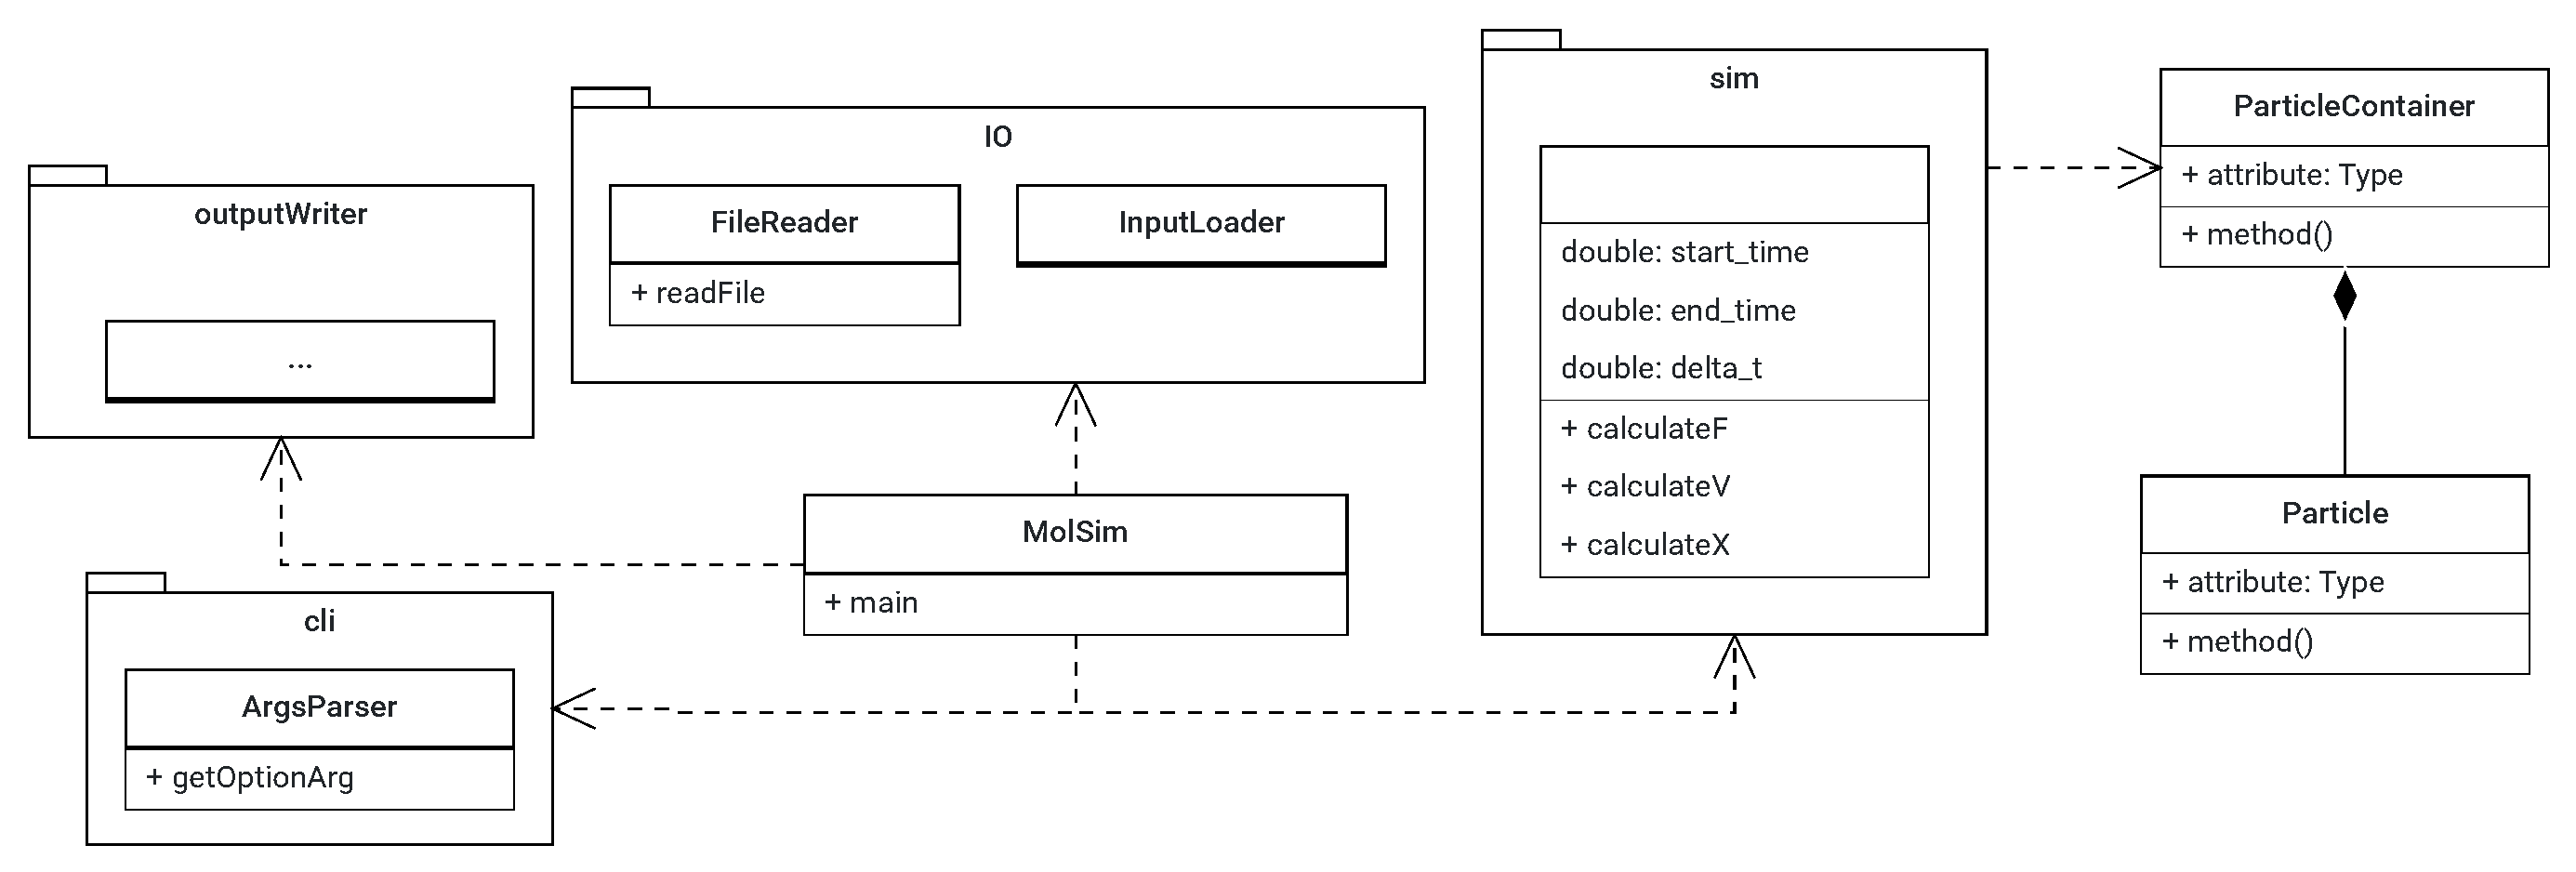
\includegraphics[height=0.5\textheight]{./UMLClassDiagram-1}
	\label{fig:umlclassdiagram-1}
\end{figure}
\end{frame}

\begin{frame}[fragile]
	\frametitle{Use of the Program}
	\vspace{0.7cm}
	\begin{Verbatim}
❯ ./MolSim --help
Welcome to MolSim Help
Usage:
MolSim <input-files> <options>
Options:
--help, -h              Prints this screen.
-dt <value>             Sets delta time to <value>. If -dt is not specified default value is used.
-et <value>             Set end time to <value>. If -et is not specified default value is used.
-o <name>               Set base name of output files. DO NOT USE A PATH! Default is 'result'.
-of <path>              Set path to output folder. Default is ./output
	\end{Verbatim}
\end{frame}

\begin{frame}[fragile]
\frametitle{Generic IO}
\vspace{0.7cm}
\begin{lstlisting}[language=C++]
template <typename LOCATOR, void (*LOAD)(LOCATOR, std::list<Particle>&)>
class InputLoader {
	private:
	std::list<Particle> buffer;
	LOCATOR locator;
	public:
	explicit InputLoader(LOCATOR loc) : locator(loc) {}
	InputLoader(const InputLoader& i) = delete;
	void reload() { LOAD(locator, buffer); }
	void getParticles(std::vector<Particle>&buf) {...}
};
\end{lstlisting}
\end{frame}

\begin{frame}
    \frametitle{Refactoring surprises}
		\large
		\begin{itemize}
			\item<1-> Task: Verify the correctness of the program after major refactoring
			\item<2-> Idea: string-compare the new output with the old output, if the program works as intended it should be the same
			\item<3-> Observation: Minuscule differences in the outputs generated (unobservable in the videos)
		\end{itemize}
		\visible<4->{What happened:}
		\begin{itemize}
			\item<5-> Floating point operations are not associative $\rightarrow$ both outputs were ``correct''
			\item<6-> Probably some compiler magic
			\item<7-> First-hand encounter with the inaccuracies of numerical programming
		\end{itemize}

\end{frame}
\clearpage

\begin{frame}
	\frametitle{bloopers}
	\includemedia[
	activate=pagevisible
	]{broken0.swf}
	\includemedia[
	activate=pagevisible]{broken1.swf}
\end{frame}

\begin{frame}
	\frametitle{Ideas, Roadblocks and Pain}
	\large
	\begin{itemize}
		\item<1-> Custom CSS Doxygen didn't cooperate
		\item<2-> Disproportion of time invested $\leftrightarrow$ relevance
		\item<3-> libxerces, Eigen deployment pain
		\item<4-> Cmake, Doctest details
		\item<5-> Iterator-related debate
		\item<6-> Data structure locality (for later exercises)
	\end{itemize}
	
\end{frame}
%%%%%%%%%%%%%%%%%%%%%%%%%%%%%%%%%%%%%%%%%%%%%%%%%%%%%


%%%%%%%%%%%%%%%%%%%%%%%%%%%%%%%%%%%%%%%%%%%%%%%%%%%%%%%%%%%%%%%%%%%%%%%%%%%%%%%%
% FOLIENSTIL: Standard mit Lehrstuhl-, Fakultäts- und Universitätsnamen im
% Kopfbereich links
\PraesentationMasterKopfzeileDreizeiler

\PraesentationTitelseite


%%%%%%%%%%%%%%%%%%%%%%%%%%%%%%%%%%%%%%%%%%%%%%%%%%%%%%%%%%%%%%%%%%%%%%%%%%%%%%%%
% FOLIENSTIL: Weisse Schrift auf blauem Grund
\PraesentationMasterWeissBlau

%%%%%%%%%%%%%%%%%%%%%%%%%%%%%%%%%%%%%%%%%%%%%%%%%%%%%
%% Startseiten                                     %%

% Setzt die Startseite auf eine mit Flaggen als Hintergrund:
\PraesentationStartseiteFlaggen

% Setzt die Startseite auf eine mit mit einer Zeichnung des TUM-Uhrenturms:
%\PraesentationStartseiteUhrenturm

% Setzt die Startseite auf eine ohne Hintergrund:
%\PraesentationStartseiteLeer

\PraesentationTitelseite % Fügt die Startseite ein
%%%%%%%%%%%%%%%%%%%%%%%%%%%%%%%%%%%%%%%%%%%%%%%%%%%%%


\begin{frame}
    \PraesentationUeberschriftZweizeilig{Präsentationsmuster}{kann auch als Kapiteltrenner verwendet werden}
\end{frame}

%%%%%%%%%%%%%%%%%%%%%%%%%%%%%%%%%%%%%%%%%%%%%%%%%%%%%%%%%%%%%%%%%%%%%%%%%%%%%%%%
% FOLIENSTIL: Weisse Schrift auf schwarzem Grund
\PraesentationMasterWeissSchwarz

\begin{frame}
    \frametitle{Präsentationsmuster}
\end{frame}


%%%%%%%%%%%%%%%%%%%%%%%%%%%%%%%%%%%%%%%%%%%%%%%%%%%%%%%%%%%%%%%%%%%%%%%%%%%%%%%%
\end{document} % !!! NICHT ENTFERNEN !!!
%%%%%%%%%%%%%%%%%%%%%%%%%%%%%%%%%%%%%%%%%%%%%%%%%%%%%%%%%%%%%%%%%%%%%%%%%%%%%%%%

